\section{Vorgehen}
\label{sec:design}

Im Rahmen der Praktikumsaufgabe werden \hyperref[sec:approaches]{verschiedene Vorgehensweisen}
zur Lösung des Entity-Resolution-Problems untersucht.
Um die Vergleichbarkeit der Ansätze zu wahren und eine größere Bandbreite von Auswertungen durchführen zu können,
wollen wir stets Standard-Java-Klassen verwenden.
Dabei sind insbesondere verschiedene Implementierungen der
\href{https://docs.oracle.com/javase/7/docs/api/java/util/List.html}{List-} und
\href{https://docs.oracle.com/javase/7/docs/api/java/util/Set.html}{Set-Schnittstellen} aus dem
\href{http://docs.oracle.com/javase/7/docs/technotes/guides/collections/overview.html}{Collections-Framework}
sowie \href{https://docs.oracle.com/javase/7/docs/api/java/security/MessageDigest.html}{MessageDigest}
und \href{https://docs.oracle.com/javase/7/docs/api/java/util/BitSet.html}{BitSet} relevant.

Zur Lösung der Aufgabe implementieren wir ein Programm (z.Bsp.: PersonEntityResolution.jar), welches für eine Ausführung
die ähnlichen Personen in zwei Personendatensätzen findet.
Dabei soll das Programm durch seine Parametrisierung flexibel aus den oben vorgestellten Lösungsansätzen, inklusive relevanter Details,
wählen können.

Zur vereinfachten Auswertung wird dieses Programm dann durch ein Skript (z.Bsp.: run\_evaluations.sh)
sequentiell für alle interessanten Konstellationen ausgeführt.
Die entstehenden Metadaten sowie Ergebnisse werden aufgehoben.
\refnice{Abbildung}{fig:workflow} stellt dieses Vorgehen schematisch dar.

\begin{figure}[h]
	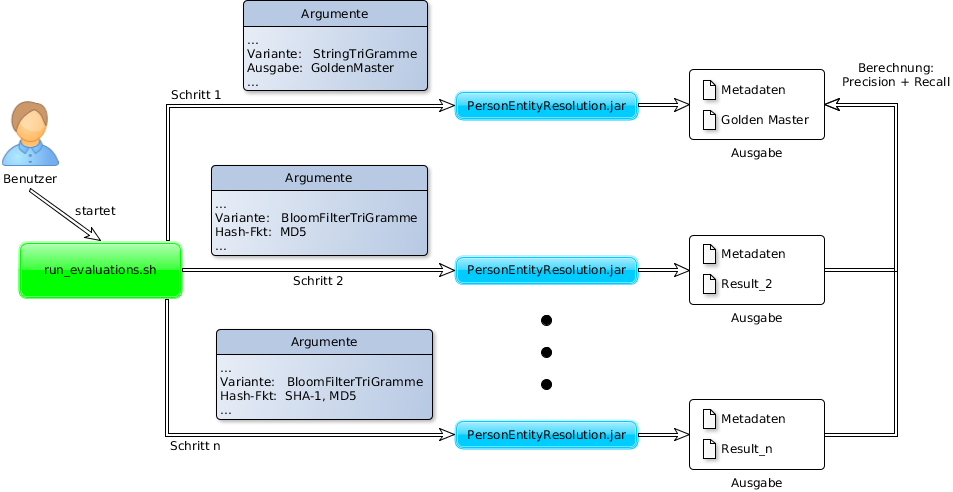
\includegraphics[width=1.01 \textwidth]{evaluation_sketch.png}
	\caption{Workflow zur Evaluierung verschiedener Entity-Resolution-Ansätze}
	\label{fig:workflow}
\end{figure}

So wird im ersten Schritt die Entity-Resolution in der ursprünglichen Variante mit \hyperref[sec:approaches:n-gramm]{String-N-Grammen} durchgeführt.
Die dabei gefundenen Paare von ähnlichen Personen werden für die Ausführungen anderer Konstellationen als Golden-Master abgelegt.

Alle weiteren Ausführungen (2 bis n) stellen nun verschiedene Varianten der Entity-Resolution mit \hyperref[sec:approaches:bloom]{Bloom-Filtern} dar.
Die Menge der anwendbaren Parameter ist vielfältig (\refnice{Abbildung}{fig:parameters} gibt eine Skizze),
was eine ausführliche Auswertung ermöglicht.
Für die Ergebnisse wird dabei stets mittels Precision und Recall gemessen, wie nah sie an die Wahrheit des Golden-Masters heranreichen.

\begin{wrapfigure}{r}{0.49\textwidth}
\begin{tabular}{|l|}
	\hline
	\begin{minipage}{0.46\textwidth}
		\vspace*{0.1cm}
		N-Gramme\\

		\hspace*{-0.4cm}
		\begin{footnotesize}
		\begin{tabular}{l|l}
				Parameter & Wertebereich\\
			\hline
			\hline
				N & TBA\\
			\hline
				Set & $\{$ HashSet, LinkedHashSet $\} \hspace*{0.34cm}$\\
		\end{tabular}
		\end{footnotesize}
	\end{minipage}\\
	\hline
	\hline
	\begin{minipage}{0.46\textwidth}
	\vspace*{0.1cm}
	Bloom-Filter\\

	\hspace*{-0.4cm}
	\begin{footnotesize}
		\begin{tabular}{l|l}
				Parameter & Wertebereich\\
			\hline
			\hline
				N & TBA\\
			\hline
				Attributschachtelung & $\{$ Ja, Nein $\}$\\
			\hline
				Länge Bitliste & \\
			\hline
				Hash-Funktionen & $\{$MD5, SHA, ...$\} \hspace*{0.53cm}$\\
		\end{tabular}
		\end{footnotesize}
	\end{minipage}\\
	\hline
\end{tabular}
\caption{Skizze möglicher Parameter}
\label{fig:parameters}
\end{wrapfigure}

Zusätzlich müssen weitere Kennzahlen erhoben werden.
Dazu gehören im Wesentlichen gemonitorte Details wie Ausführungszeiten und der benötigte Speicherplatz.
Auf Basis der so gesammelten Informationen können ausgiebige Vergleiche der verwendeten Ansätze durchgeführt werden.

Gleichzeitig ist der in \refnice{Abbildung}{fig:workflow} dargestellte Ansatz flexibel genug,
um ohne zusätzlichen Aufwand Tests mehrfach auszuführen und somit Seiteneffekte auszuschließen.
